\chapter{서론}
\label{sec:introduction}

% A:아내, B:남편
\newcommand{\A}{지효}
\newcommand{\B}{승표}


% 교수님 커멘트 Problem & Solution approach가 명확하지 않은 글. 
% 이것을 좀 더 강화해야
% problem이 뭔지? solution approach가 뭔지?

%%%% 1번째 단락: 은근한 함께함 체험시키기 시나리오 %%%%
%%%% --------------------------------------------------

% 시나리오 버전 1
% 도시에서 바쁜 일상을 살아가는 부부인 \A와 \B를 생각해보자. 그들은 각자의 직장에서 바쁜 한 주를 보낸 후, 마침내 주말을 맞이하였다. \B는 모처럼 아내와 즐거운 시간을 보내기 위해 야심차게 데이트를 준비했지만, 여전히 일이 남은 \A는 주말에도 집에서 업무를 해야 했다. 어쩔 수 없이 \B는 바쁜 아내를 위해 커피를 같이 마시고 옆에서 책을 읽으며 토요일 오후를 보내게 되었다. \B는 비록 아내와 계획했던 데이트를 하지는 못했지만, 아내와 주말 오후를 같이 보내며 잔잔한 만족감을 느꼈다. \A는 바쁘게 일을 하면서도, 자신의 옆에 같이 있어준 남편 덕분에 편안함과 안정감을 느꼈다. 이들은 서로에게 집중하지도, 같은 활동을 하지도, 긴 대화를 나눈 것도 아니었지만, 편안하고 잔잔하게 느껴지는 `\concept'을 즐기며 더 깊은 유대감을 만들고 행복한 기억을 만들었다. \highlight{이후 두 사람은 \A가 바쁜 주말을 보내야 할 때마다 자주 이러한 시간을 보내곤 했다.} 그런데 어느 날, \A는 직장에서 미국 지사로 발령받았고 \A와 \B는 결국 떨어져 살게 되었다. 같이 살 때의 마음을 이어가기 위해 그들은 서로 자주 통화하고 꾸준히 대화를 했지만, 그들은 자주 집에 같이 보냈던 토요일 오후가 그리웠다. 이 부부는 더 이상 `\concept'을 느낄 수 없게 된 것일까?

% 시나리오 버전 2
%맞벌이 부부 \A와 \B는 각자 업무에 치여 정신없는 한 주를 보낸 뒤 토요일을 맞이하였다. 그들은 모처럼 달콤한 데이트를 하기 위해 놀이공원에 갈 계획 이었으나, 이는 일장춘몽에 불과했다. 토요일 아침 \A의 상사로부터 걸려 온 전화, 이로 인해 \A는 꼼짝없이 집에서 일을 해야만 했다. 어쩔 수 없이 \B는 바쁜 아내를 위해 커피를 같이 마시고 옆에서 책을 읽으며 토요일 오후를 보냈다. \B는 비록 아내와 계획했던 달콤한 데이트를 하지는 못했지만, 아내와 주말 오후를 같이 보내며 잔잔한 만족감을 느꼈다. \A는 바쁘게 일을 하면서도, 자신의 옆에 같이 있어준 남편 덕분에 편안함과 안정감을 느꼈다. 이들은 서로에게 집중하며 활동적인 데이트를 즐긴 것도, 긴 대화를 나눈 것도 아니었지만, 편안하고 잔잔하게 느껴지는 `\concept'을 즐기며 더 깊은 유대감을 만들고 좋은 기억을 만들었다. \highlight{이후 두 사람은 \A가 바쁜 주말을 보내야 할 때마다 자주 이러한 시간을 보내곤 했다.} 그런데 어느 날, \A는 직장에서 미국 지사로 발령받았고 \A와 \B는 결국 떨어져 살게 되었다. 같이 살 때의 마음을 이어가기 위해 그들은 서로 자주 통화하고 꾸준히 대화를 했지만, 그들은 종종 집에서 같이 보냈던 토요일 오후가 그리웠다. 이 부부는 더 이상 `\concept'을 느낄 수 없게 된 것일까?

%시나리오 버전 3
맞벌이 부부이자 독서를 좋아하는 \B\와 \A에게 느긋하게 커피를 마시며 함께 책을 읽는 토요일 오후는 \concept\을 느끼는 매우 소중한 시간이다. 정신없이 바쁜 직장생활 때문에 혼자인가 싶다가도, 이 시간을 통해 서로 함께하고 있다는 것을 다시금 확인하게 된다. 사실 많은 대화가 오고 가는 시간은 아니다. 그들은 각자 자신의 책을 읽는데 집중한다. 그렇지만, 하고 싶은 일을 마음껏 하면서도 사랑하는 사람이 곁에 있다는 점과 언제든 자신의 생각을 공유할 상대가 있다는 점이 \A\와 \B에게는 큰 편안함과 안정감을 준다. 잔잔하게 느껴지는 \concept\은 그들의 관계를 더욱 돈독하게 만들어왔다. 그러던 어느 날, 이 부부에게 청천벽력 같은 소식이 떨어졌다. \A\가 직장에서 미국 지사로 발령받아 더 이상 이 토요일 오후 시간을 함께 할 수 없게 된 것이다. 함께 책을 읽던 시간을 떠올리며 통화를 하지만, 그들은 종종 집에서 같이 보냈던 토요일 오후가 그리웠다. 이 부부는 더 이상 `\concept'\을 느낄 수 없게 된 것일까?

%%%% 2번째 단락: 문제 제기 %%%%
%버전 1 --> 기존의 연구들과 비교를 좀 해줘야 하지 않을까?
\A\와 \B\ 부부처럼, 직장 혹은 학업 때문에 어쩔 수 없이 떨어져 살게 되는 가족은 전세계적으로 늘어나고 있다. 현재 미국에만 총 360만 명의 부부가 떨어져 살고 있으며, 영국의 경우에도 전체 부부의 10\%가 떨어져서 살고 있다 \cite{duncan2013people, strohm2009living}. 이는 한국도 크게 다르지 않은데, 비동거 맞벌이 가구 수는 전체 가구의 4.6\%에 달하며, 서울의 경우 10쌍 중 1쌍이 기러기 가족 생활을 하고 있다 \cite{rock2016goose, wise2012seoul}. 이들은 인터넷 및 IoT 기술의 발전으로 메신저, 영상통화, 소셜 미디어 등을 통해 서로 연락하기 쉬워졌지만, 여전히 \A\와 \B\ 부부가 함께 있을 때 느꼈던 \concept\을 느낄 수 없고 이로 인한 아쉬움과 그리움을 떨쳐 낼 수가 없다.
\tglee{충국이형: 왜 통화로 할 수 없었는지를 elaborate 하면 좋지 않을까}비록 물리적으로 떨어져 있지만, 그럼에도 같이 살았을 때의 \concept\을 만들어 줄 수는 없을까? 

%버전 2 --> 메신저, 영상통화, 소셜미디어 빼고 기존의 연구들 두 문장 추가함. 너무 추상적인 것 같기도...
%\A와 \B\ 부부처럼, 직장 혹은 학업 때문에 어쩔 수 없이 떨어져 살게되는 가족은 전세계적으로 늘어나고 있다. 현재 미국에만 총 360만명의 부부가 떨어져 살고 있으며, 영국의 경우에도 전체 부부의 10\%가 떨어져서 살고 있다 \cite{strohm2009living, duncan2013people}. 이는 한국도 크게 다르지 않은데, 비동거 맞벌이 가구 수는 전체 가구의 4.6\%에 달하며, 서울의 경우 10쌍 중 1쌍이 기러기 가족 생활을 하고 있다 \cite{rock2016goose, wise2012seoul}. 학계에서는 이러한 가족들에게 함께함(co-presence)을 경험하게 하는 것을 중요한 문제로 여기고 활발히 연구하고 있다. 하지만, 기존의 연구들은 대부분 특정 활동을 함께 할 때 경험하게 되는 함께함에 초점이 맞추어져 있다 \cite{kirk2010home, neustaedter2012intimacy, judge2010sharing, yang2017communicating}. 이는 \A와 \B부부가 상대방을 은근하게 느끼면서 경험하던 \concept과는 다른 종류의 함께 함이다. 


%%%% 3번째 단락: solution approach 1 %%%%

%%%%%%%%%%%%%%%%%%%%%%%%%%%%%%%%%%%%%%%%%%%%%%%%%%%%%%%%%%%%%%%%%%%%%%%%%
\begin{figure}
\begin{subfigure}{.5\textwidth}
  \centering
  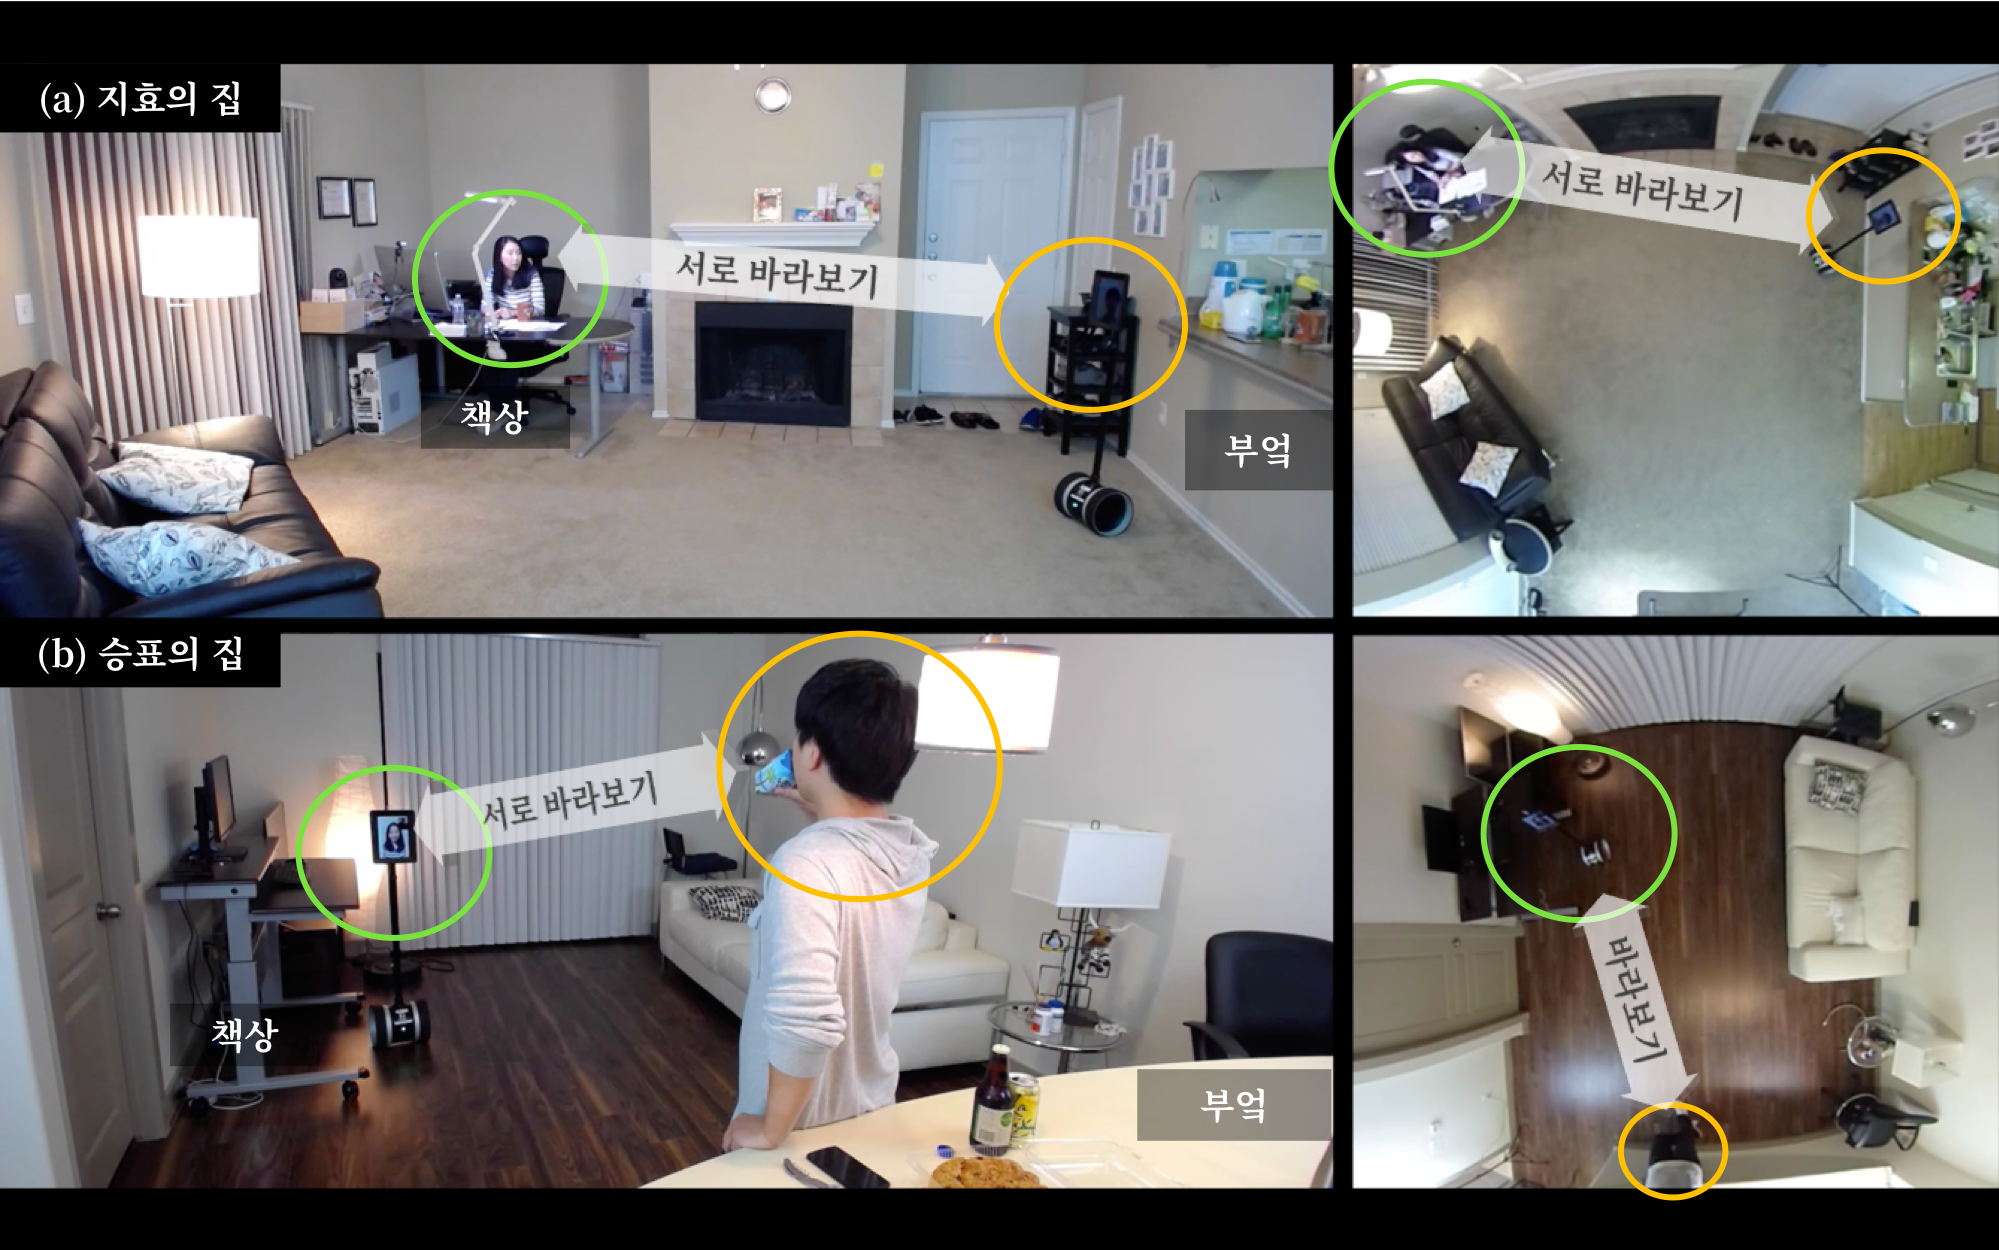
\includegraphics[width=\textwidth]{images/concept1}
\end{subfigure}
\begin{subfigure}{.5\textwidth}
  \centering
  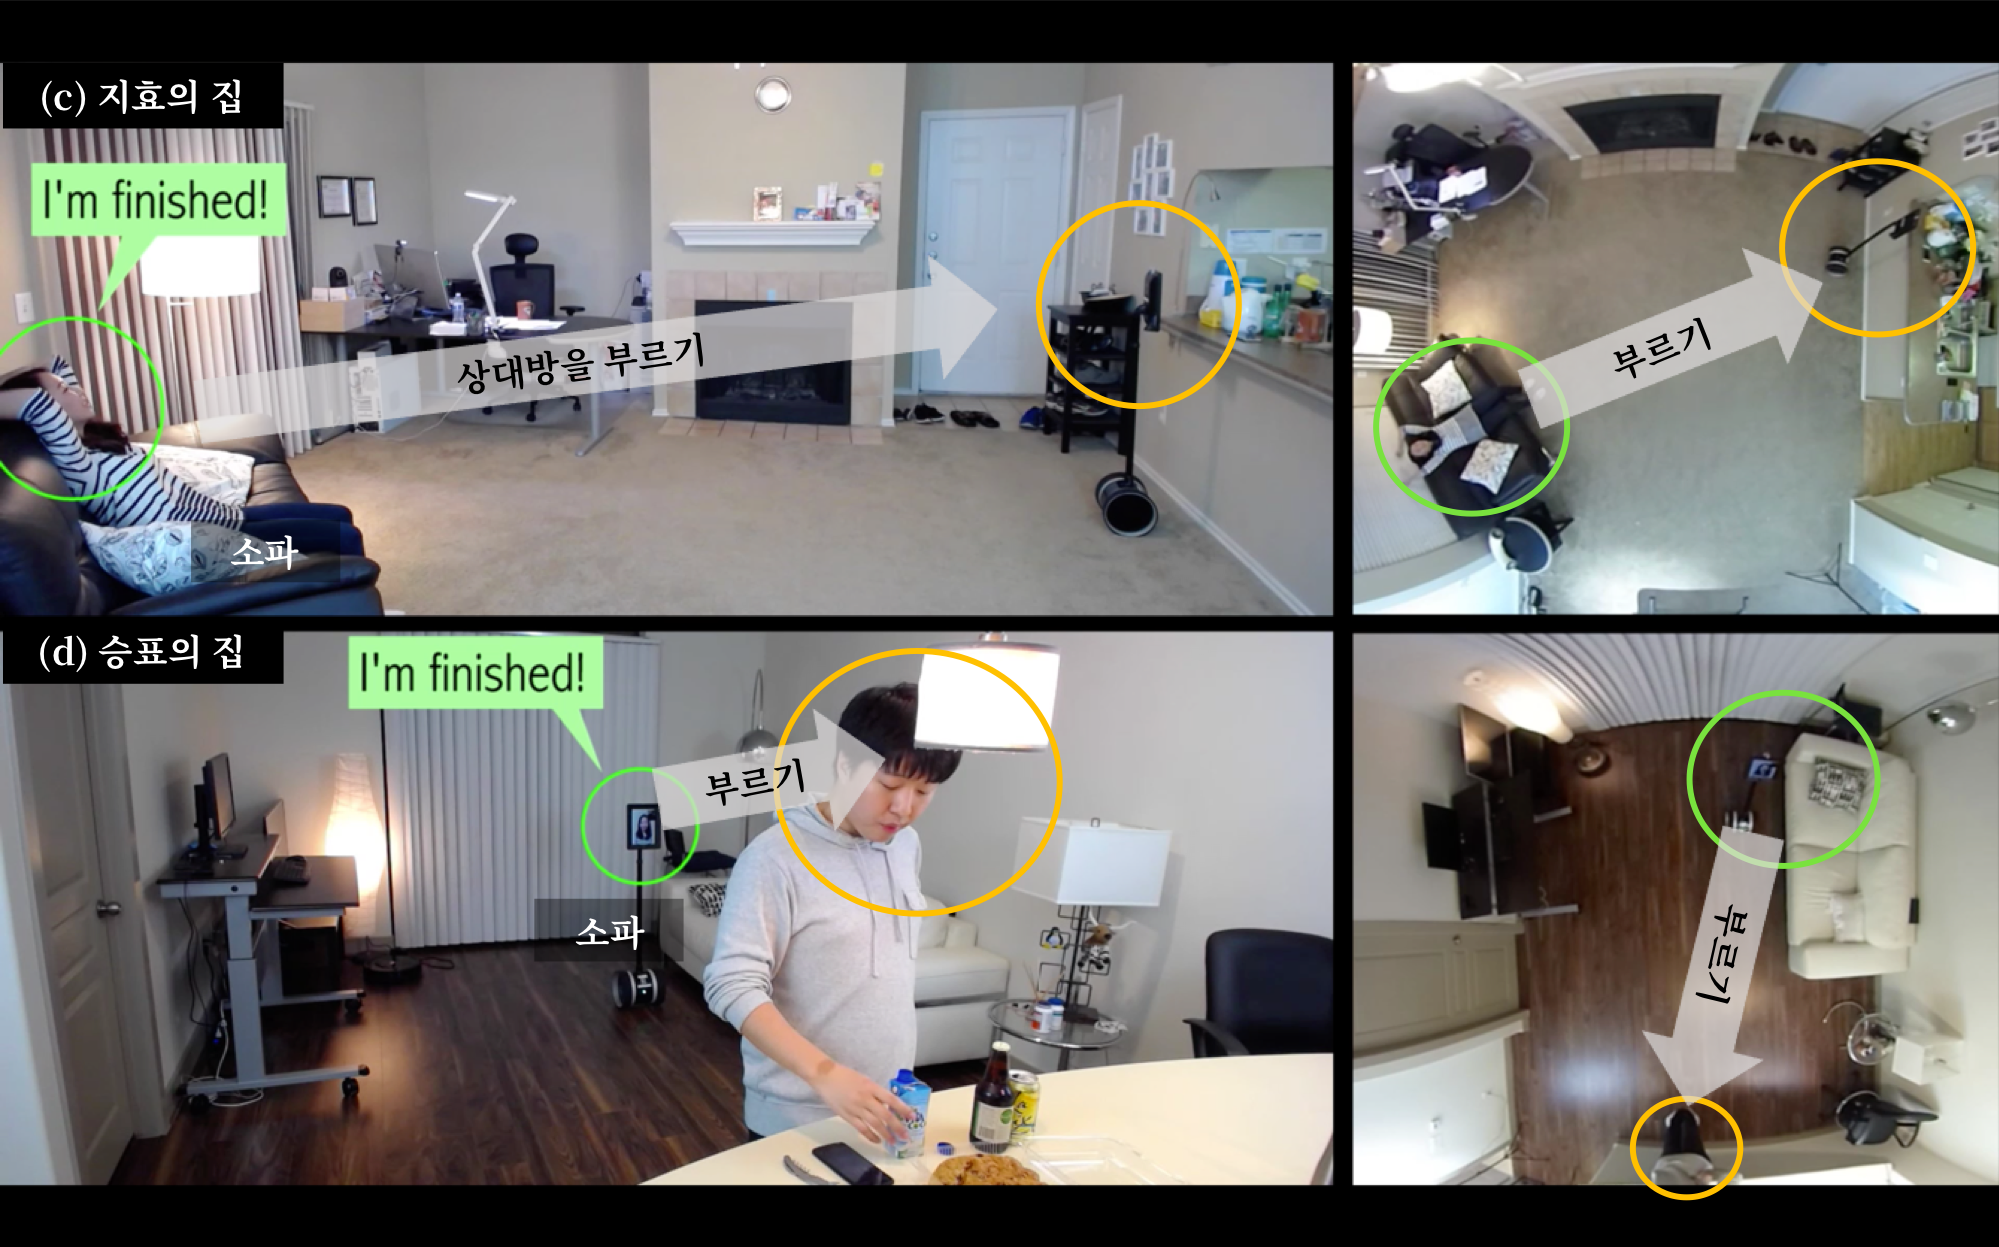
\includegraphics[width=\textwidth]{images/concept2}
\end{subfigure}
\caption{\approach을 이용한 시스템의 콘셉트}
\label{fig:concept}
\end{figure}
%%%%%%%%%%%%%%%%%%%%%%%%%%%%%%%%%%%%%%%%%%%%%%%%%%%%%%%%%%%%%%%%%%%%%%%%%

% 버전1
% 나는 서로 떨어져 사는 가족들에게 \concept을 제공하기 위한 하나의 방법으로 로봇 아바타 기반 항시적 위치 동기화 방식, \sysname를 제시한다. \sysname는 떨어져 사는 두 사람을 각자의 집에 투영하여 \concept을 제공하고자 각각 서로를 대변하는 아바타로써 텔레프레즌스(Telepresence) 로봇\cite{double_robotics}을 사용한다. 집 A에 있는 사람의 로봇 아바타가 집 B에 있고, 집 B에 사는 사람의 아바타가 집 A에 있으며, 이 로봇 아바타는 상대방의 집안 위치와 의미적으로 유사한 곳에 위치한다. 즉, 집 B 에 사는 상대방이 소파에서 TV 를 보다가 화장실로 움직이면, 집 A에서 소파에 있다가 화장실로 이동한다. 사용자들은 로봇 아바타를 통해 상대방의 집안 움직임과 위치를 직관적으로 파악하고 이를 통해 상대방의 행동과 상태를 쉽고 자연스럽게 알 수 있게 된다. 예를 들어, 로봇 아바타가 집안 냉장고 앞에 있다면, 상대방이 냉장고에서 음식이나 음료를 찾는 중이라는 것을 알 수 있다.

%버전2 --> 집 A, 집 B를 없애고 싶었음.
% 본 연구에서 나는 서로 떨어져 사는 가족들에게 \concept\을 제공하기 위한 하나의 방법으로 `\approach'\을 제시한다. 이는 텔레프레젠스 로봇(Telepresence Robot \cite{double_robotics})이 상대방의 아바타가 되어, 
% \highlight{내 집에서 상대방의 위치를 나타내는 방식이다.}
% 상대방이 소파에서 TV를 보다가 화장실에 가면, 내 집에 있는 상대방의 로봇 아바타도 소파에 있다가 화장실로 움직이게 된다. 사용자들은 로봇 아바타를 통해 상대방의 움직임과 위치를 직관적으로 파악하고, 이를 통해 상대방의 행동과 상태를 쉽고 자연스럽게 알 수 있다. 예를 들어, 로봇 아바타가 집안 냉장고 앞에 있다면, 상대방이 냉장고에서 음식이나 음료를 찾는 중이라는 것을 알 수 있다.

% 버전3 교수님과 연구실 사람들과 같이 고쳐봄
본 연구에서는 이를 실현할 수 있는 한 가지 방법으로 `\approach'\을 제시한다. 이는 텔레프레즌스 로봇(Telepresence Robot \cite{double_robotics})을 상대방의 아바타로 삼고 내 집 적절한 장소에 놓아, 상대방의 행동과 상황을 잘 표현하는 방식이다. 떨어져 사는 상대방의 행동을 가장 비슷하게 나타낼 수 있는 내 공간상의 장소에 위치하는 아바타를 상상해보자. 예를 들어, 상대방이 집에서 먹을 음식을 찾고 있으면, 아바타는 냉장고 앞에 위치하게 된다. 사람들은 이러한 아바타를 통해 상대방의 행동을 쉽게 유추하고 \concept\을 느낄 수 있을 것이다.


%%%% 4번째 단락: solution approach 2 %%%%
%제안하는 방식이 어떻게 또는 왜 \concept을 제공할 수 있는지 한문단.

% 버전1
% \approach의 핵심 요소는 `텔레프레즌스 로봇의 활용'과 `의미적으로 유사한 위치 및 방향(semantically equivalent location/orientation)의 재현'이다.
% \tglee{충국이형: 두 요소가 독립적인가? 같은 level 이 아닌 것 같음}
% 이는 떨어져 산 경험이 있는 가족 구성원들을 대상으로 진행한 \expWorkshop\을 통해 도출되었다.
% 텔레프레즌스 로봇의 활용은 물리적인 실체를 통해 상대방의 존재와 인기척을 효과적으로 나타내며, 사용자에게 장비 착용을 요구하지 않기에 일상에서 이를 지속적으로 사용하는 것을 가능케 한다.
% 또한, 의미적으로 유사한 위치와 방향의 재현은 상대방의 행동과 상태를 쉽게 전달하고 이를 사용자들이 인지하는데 큰 노력과 집중을 들이지 않도록 만든다. \highlight{이처럼 상대방을 나타내는 로봇 아바타는 자연스럽게 사용자의 일상에 녹아들어 `\concept'\을 연출한다.}

% 버전2
\approach의 핵심 요소는 `의미적으로 유사한 위치 및 방향(semantically equivalent location/orientation)의 재현'이다.
이는 떨어져 산 경험이 있는 가족 구성원들을 대상으로 진행한 \expWorkshop\을 통해 도출되었다.
먼저, 본 연구에서는 \concept을 제공하기 위한 합리적인 디자인 요소로써 텔레프레즌스 로봇을 선택하였다.
로봇의 사용은 물리적인 실체를 통해 상대방의 존재와 인기척을 효과적으로 나타내며, 사용자에게 장비 착용을 요구하지 않기에 일상에서 이를 지속적으로 사용하는 것을 가능케 한다.
이러한 로봇의 활용은 이를 어떤 장소에 위치시키는가에 대한 질문으로 연결된다. 이에 본 연구는 \expWorkshop을 통해 얻은 `의미적으로 유사한 위치와 방향의 재현'을 제안한다.
로봇을 통해 가구중심을 기반으로 의미적으로 유사한 위치와 방향을 재현하는 것은 상대방의 행동과 상태를 쉽게 전달하고 이를 사용자들이 인지하는데 큰 노력과 집중을 들이지 않도록 만든다. \highlight{이는 자연스럽게 사용자의 일상에 녹아들어 `\concept'\을 연출한다.}


% 이를 토대로 `\approach'를 고안하였으며 각 핵심요소는 다음과 같이 \concept을 제공한다.
% (1) 물리적인 실체가 있는 로봇의 활용은 상대방의 존재와 인기척을 효과적으로 나타내며,
% (2) 의미적으로 유사한 위치와 방향을 재현함으로써 상대방의 행동과 상태를 쉽게 전달한다. 또한, 
% (3) 로봇의 위치와 움직임을 통해 상대방의 맥락을 전달하기 때문에 이를 사용자들이 인지하는데 큰 노력과 집중이 요구되지 않으며 일상에 은근하게 녹아들 수 있다. 마지막으로 이 방식은 사용자에게 장비착용을 요구하지 않기에, 
% (4) 사용자들이 일상에서 이를 지속적으로 사용하는 것이 현실적으로 가능하다.


% \approach의 목적은 `의미적으로 유사한 위치(semantically equivalent location)'를 `실체가 있는 유형물'을 통해 재현하고자 함이다.
% 이는 떨어져 살아본 가족 구성원들을 대상으로 진행한 \expWorkshop에 근거한다. 제안하는 방식의 요소들은 다음과 같이 \concept을 제공한다.
% (1) 물리적인 실체가 있는 텔레프레즌스 로봇으로 상대방의 존재와 인기척을 효과적으로 나타내며,
% (2) 의미적으로 유사한 위치와 방향을 재현함으로써 상대방의 행동과 상태를 쉽게 전달한다. 또한, (3) 로봇의 위치와 움직임을 통해 상대방의 맥락을 전달하기 때문에 이를 인지하는데 큰 노력과 집중이 요구되지 않으며 사용자의 일상에 은근하게 녹아들 수 있다. 
% 마지막으로 이 방식은 사용자에게 장비착용을 요구하지 않기에, (4) 사용자들은 일상에서 이를 지속적으로 사용할 수 있다.

% 우리 방식이 동작하는 이유
% - 실체가 있는 로봇을 통해 존재감과 인기척을 잘 나타낸다
% - 의미적으로 유사한 위치를 통해 행동과 상태를 잘 전달해 준다.
% - 추상화된 로봇을 움직이는 것이기 때문에 이를 인지하는데 큰 노력이나 집중이 요구되지 않는다
% -- 이 방식은 사용자에게 장비착용을 요구하지 않는다. 이는 일상에서 지속적으로 사용되는데 용이


%%%% 5번째 단락: 실험 %%%%

본 연구에서는 제안하는 방식이 실제로 \concept을 성공적으로 형성하는지를 확인하고자 \expUser\을 진행하였다. 먼저, \approach을 실현할 수 있는 프로토타입 시스템의 구성요소를 제시하고 이를 각각 사람이 모사하는 인간참여형 시스템 \concept을 구현하였다. 이후 총 5 쌍의 실제 부부 및 커플들을 대상으로 오즈의 마법사 실험을 진행하였으며, 이를 통해 제안하는 방식의 적절성과 효과를 탐구하였다. 실험 결과, 떨어져 사는 사람들의 상대방의 상황 파악에 대한 적극성을 확인할 수 있었으며, 상대방의 위치에서 들려오는 소리, 대화의 공백에 대한 적은 부담감, 로봇의 움직임이 주는 대화의 기회 등의 요소를 긍정적으로 평가했다.


%%%% 6번째 단락: Contribution %%%%

본 연구의 의의는 다음과 같다.
먼저, 소셜 컴퓨팅 분야에 `\concept'\이라는 중요한 개념을 새롭게 제시한다.
\highlight{이는 떨어져 사는 가족들에게 적합한 새로운 장르의 원거리 인터랙션 기술 및 서비스의 지평을 연다.}
둘째, 떨어져 사는 가족들에게 \concept\을 효과적으로 제공할 수 있는 \approach\을 고안하였다.
\highlight{셋째, \concept에 대한 실험의 어려움을 정리, 이를 해결하기 위한 초기 실험 디자인을 제시한다.}
마지막으로, 인간참여형 \sysname\를 만들고 제한적인 실험환경에서 \concept의 효과를 탐구하였다.


%%%% 7번째 단락: 논문 구성 %%%%

본 논문은 아래와 같은 구성으로 이루어져 있다. \ref{sec:concept}장에서는 본 연구에서 다루는 `\concept'\이라는 개념을 소개한다. \ref{sec:design_workshop}장에서는 떨어져 사는 가족들에게 `\concept'\을 제공하는 서비스 디자인 요소를 탐구하기 위한 \expWorkshop\을 다루며, 이를 바탕으로 \ref{sec:system_design}장에서는 로봇 아바타 기반 항시적 위치 동기화 방식을 제시한다. \ref{sec:userstudy}장에서는 \sysname\를 통해 제공되는 \concept\을 관찰하기 위한 실험의 설계와 그 결과를 보여준다. \ref{sec:discussion}장에서는 본 연구에서 제시하는 디자인과 실험에 대한 논의를 다루며, \ref{sec:relatedwork}장에서는 관련된 연구들을 정리한다. 마지막으로 \ref{sec:conclusion}장에서는 본 연구의 결론을 서술한다.



% \begin{enumerate}
% \item [1] 시나리오를 던진다. (은근한 함께삶에 언제 느껴지는 건지, 얼마나 좋은 건지.) 우리는 이것을 은근한 함께 삶이라 부르려고 한다.
% \item [2] 떨어져 있는 사람들은 은근한 함께 삶을 느끼지 못한다. 과연 이들에게 은근한 함께 삶을 전달해 줄 수 있을까?
% \item [3] 우리는 이에 대한 해답으로 로봇 아바타 기반 항시적 위치 동기화 시스템, 홈멜드를 제시한다. xxx
% \item [4] 유저스터디 했다. 제한된 환경에서. finding도 써주고, 결론 breif
% \item [5] Contribution
% \begin{itemize}
%     \item (개념) CS 커뮤니티에 `은근한 함께함’ 이라는 중요한 개념을 새롭게 제시
%     \item (개발) 은근한 함께함을 제공하기 위한 `로봇 아바타 기반 항시적 위치 동기화 어프로치’ 고안/제시
%     \item (실험) evaluated.
% \end{itemize}
% \item [6] 이 논문의 구성에 대한 소개
% % 앞으로 섹션은 다음과 같이 구성된다. 3장에서는 XXX를 다룬다.
% \end{enumerate}



%%%%%%%%%%%%%%%%%%%%%%%%%%%%%%%%%%%%%%%%%%%%%%%%%%%%%%%%
% % 지구촌 -- 사람간 연결 기술의 발전
% 1964년 마셜 맥루헌이 지구촌이라는 말을 꺼낸 이후로\cite{mcluhan1994understanding}, 우리는 지구 반대편에서도 메신저, 영상통화, 소셜 미디어, 인터넷을 통해 서로 같이 얘기하고, 토론할 수 있게 되었다.
% % 아쉬움 -- 어쩔 수 없이 떨어져 사는 사람들
% 그러나 이러한 사람간 연결기술의 발전에도 아직 아쉬움을 느끼는 사람들이 있다. 직장 때문에, 학업 때문에 어쩔 수 없이 떨어져 살아가는 가족들이다. 미국에만 360만명의 부부가 떨어져 살고 있으며, 영국의 경우 전체 커플의 10\%가 서로 떨어져 산다\,\cite{strohm2009living, duncan2013people}. 
% 한국도 크게 다르지 않다. 비동거 맞벌이 가구 수는 전체 가구의 4.6\%에 달하며, 서울의 경우 10쌍 중 1쌍이 기러기 가족 생활을 하고 있다\,\cite{rock2016goose, wise2012seoul}.
% % 함께 사는 듯한 경험
% 우리는 조금 더 큰 꿈을 꾸어보려고 한다. 과연 이들에게 떨어져 있음에도 마치 함께 사는 듯한 경험을 느끼게 만들어 줄 수 있을까?
%%%%%%%%%%%%%%%%%%%%%%%%%%%%%%%%%%%%%%%%%%%%%%%%%%%%%%%%



% \begin{itemize}
% \item 함께 살 때 은근한 함께함을 느끼는 시나리오
%     \begin{itemize}
%     \item (아들의 움직임 / 잔소리) \\
%     야밤에 야식을 먹으러 살금살금 주방에 가던 아들을 TV 를 보던 엄마가 발견.
%     밤에 무슨 라면이냐며, 살금살금가면 내가 모를줄 알았냐며 하는 잔소리
%     \item (부인의 숨소리 / 피로한 사람을 위한 배려) \\
%     남편은 부엌 식탁에서 일하는 중. 점점 TV소리 사이사이에 숨소리가 커짐. 남편은 부인을 깨우지 않고 이불을 덮어줌.
%     \item (웃는 동작·소리 / 커플의 한적한 시간 보내기) \\
%     서로 소파에 누워서 핸드폰 하기
%     여자친구의 피식거리는 웃음소리를 남자친구가 봄.
%     “뭐야” 하면서 발로 툭 건드림. 같이 유튜브 영상을 봄
%     \end{itemize}
% \item 우리는 해당 경험들을 “은근한 함께함”으로 정의한다.
% \item 하지만 이런 은근한 함께함은 떨어져 살게 되면 느낄 수 없다.
%     \begin{itemize}
%     \item 우리는 토론하려고 가족을 만든 게 아니다. 가족끼리 잘 사는 모습이, 정해진 시간에 자리에 앉아서 서로서로 하루 일과와 의견을 교환하는 것은 아니다.
%     \item 어쩔 수 없이 떨어져 사는 사람들이 느끼는 아쉬움 (다양한 기술들이 있지만 부족하다)
%     \item 은근한 함께함의 요소
%     \end{itemize}
% \item 은근한 함께함을 위한 서비스 디자인 요소들을 뽑아 보았고 
% \item 로봇 아바타 시스템 프로토타입으로 실험해 봄 --- findings
% \item Contribution
%     \begin{itemize}
%     \item (개념) ‘은근한 함께함’ 이라는 새로운 개념을 정의
%     \item (개발) 은근한 함께함을 제공하기 위한 ‘로봇 아바타 기반 항시적 위치 동기화 어프로치’ 고안/제시
%     \item (실험) 구현하고 evaluated.
%     \end{itemize}
% \end{itemize}

